% -------------------------------------------------------
%  Section 11: Critical re-assessment of our own results
% -------------------------------------------------------
\section{بازارزیابی انتقادی نتایج خودمان}
\label{sec:reassess}

اگر قرار است نقد \S\ref{sec:critique} جدی گرفته شود، باید همان سخت‌گیری را درباره کار خودمان هم به کار بست.

\subsection{نقصی در پروتکل ارزیابی و اصلاح آن}
تابع آموزش، مجموعه فایل‌ها را با تفکیک ۸۰ به ۲۰ لایه‌ای می‌شکند، ولی سنجه‌های اصلی (صحت، \lr{F1} کلان، \lr{MCC}، گزارش درون‌کلاسی و ماتریس درهم‌ریختگی) روی \emph{کل} \num{۲۷٬۵۷۱} نمونه محاسبه می‌شدند، چون بارگذار ارزیابی روی همه فایل‌ها ساخته شده بود. سنجه حاصل میانگین وزن‌داری میان حافظه مدل و تعمیم آن است و دقیقاً بازسازی‌پذیر است؛ برای بهترین مدل چرخه سوم:
\begin{equation}
    0.8 \times 83.52 + 0.2 \times 65.26 = 79.87
\end{equation}
و برای \lr{VGG16} روی \lr{S3} به‌صورت $0.8 \times 86.19 + 0.2 \times 31.22 = 75.19$. یعنی عدد \pct{۷۵٫۱۹} برای \lr{VGG16} تقریباً به‌تمامی از حفظ کردن داده آموزش می‌آید و صحت واقعی آن روی داده دیده‌نشده \pct{۳۱٫۲۲} است.

برای اصلاح، تفکیک اصلی را با همان بذر و ترتیب فایل‌ها بازسازی و همه سنجه‌ها را برای هر ۸۵ اجرا از نو محاسبه کردیم؛ درستی بازسازی با تطبیق تا چهار رقم اعشار با مقادیر اعتبارسنجی ثبت‌شده تأیید شد. تمام اعداد جدول‌های \ref{tab:armbase} و \ref{tab:armopt} خروجی همین محاسبه‌اند و شکل \ref{fig:gap} اندازه شکاف را نشان می‌دهد.

\begin{figure}[!ht]
    \centering
    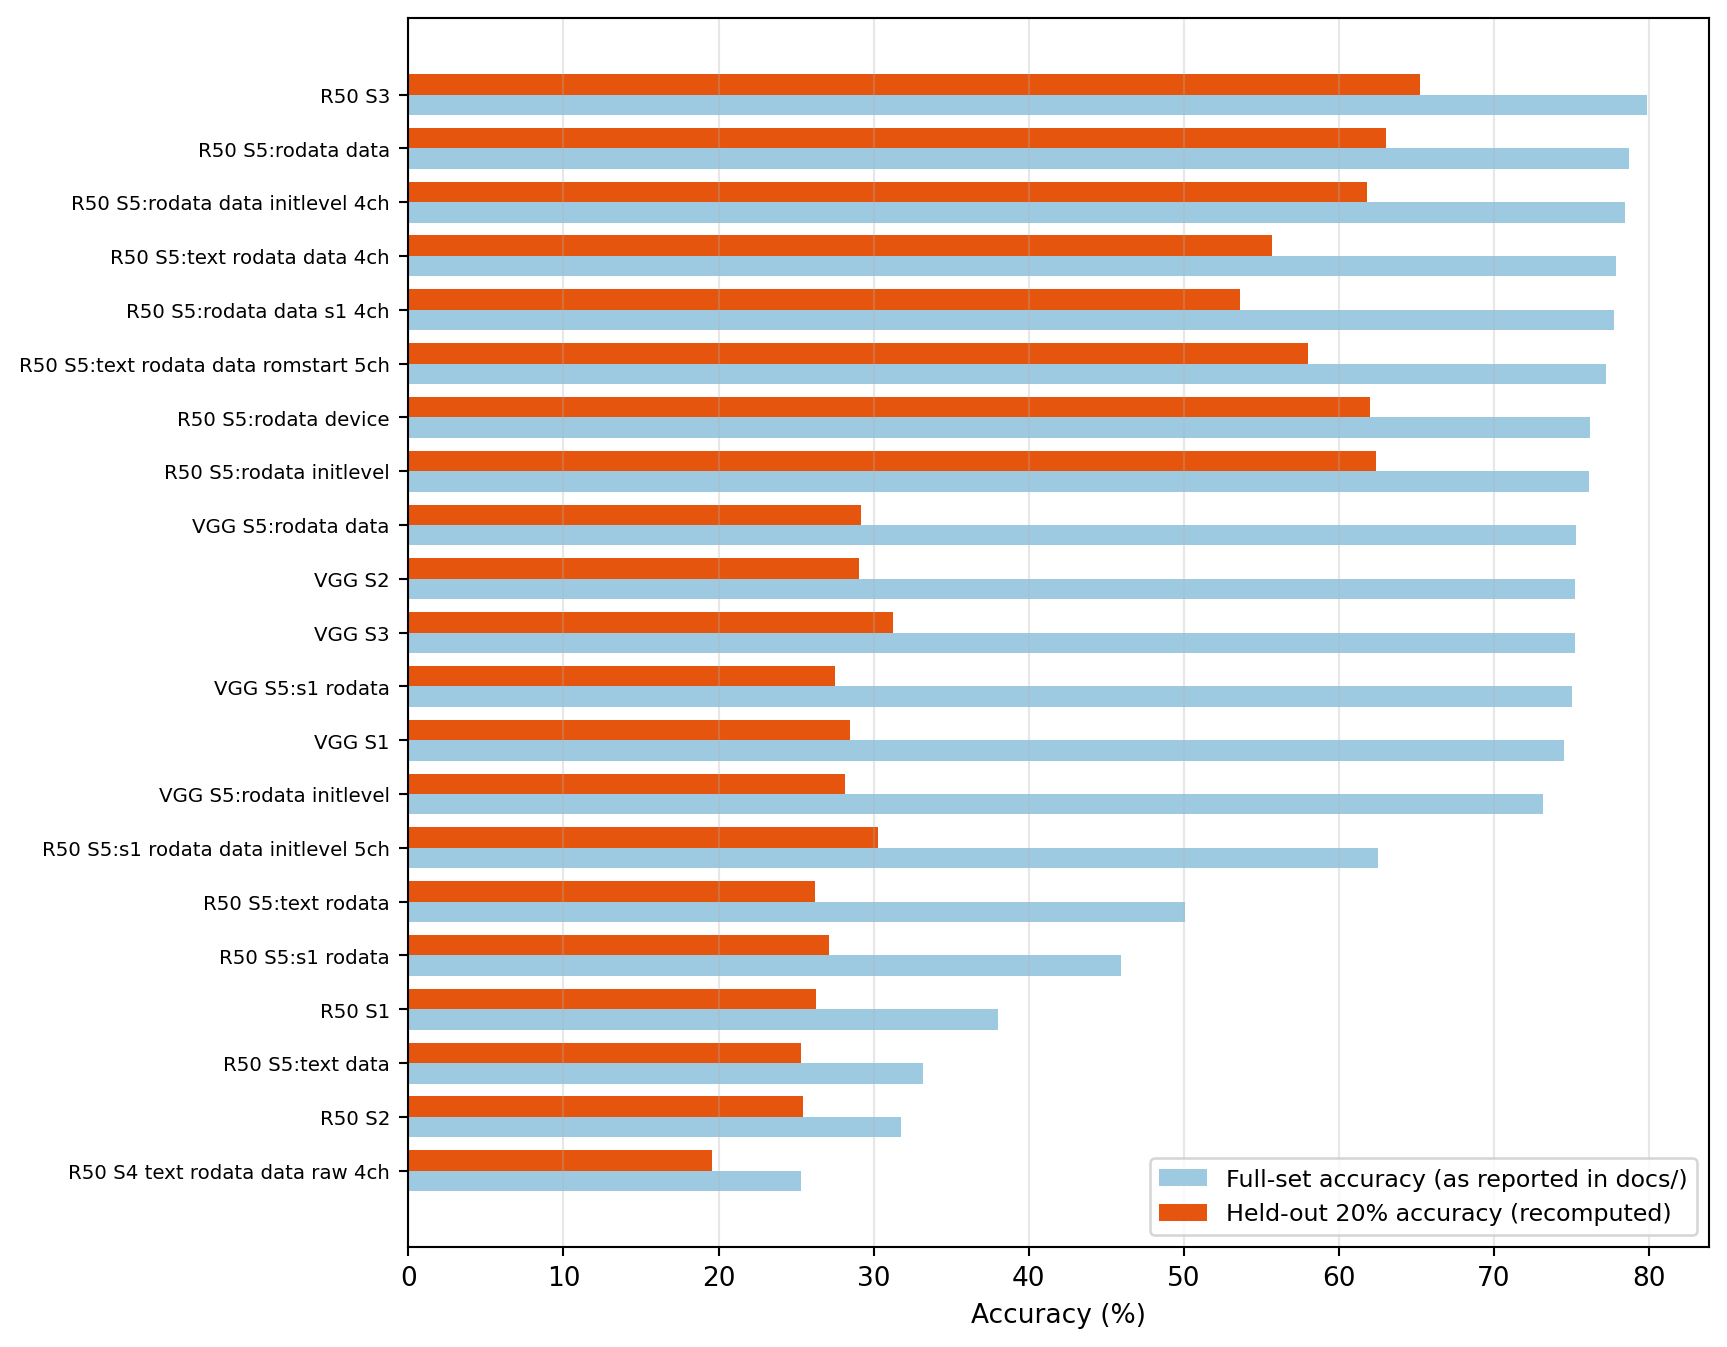
\includegraphics[width=0.56\textwidth]{figs/holdout_gap.png}
    \caption{شکاف میان صحت کل‌داده و صحت روی \pct{۲۰} نگه‌داشته‌شده، برای ۲۱ پیکربندی چرخه سوم. شکاف در پیکربندی‌های \lr{VGG16} از ۴۰ واحد فراتر می‌رود.}
    \label{fig:gap}
\end{figure}

\subsection{آیا بهبود‌های فاز چهارم واقعاً بهبود بودند؟}
دوازده پیکربندی میان چرخه اول و چرخه سوم مشترک‌اند و مقایسه زوجی آن‌ها پاسخ روشنی می‌دهد: صحت کل‌داده به‌طور میانگین \num{۵٫۰۱} واحد بالا رفته، ولی صحت روی داده نگه‌داشته‌شده به‌طور میانگین \num{۴٫۹۰} واحد پایین آمده و این کاهش در هر ۱۲ پیکربندی بدون استثنا رخ داده است. یعنی افزایش بودجه آموزش از ۲۰ به ۳۰ دوره عمدتاً ظرفیت حفظ داده آموزش را افزوده است.

با این حال نتیجه‌گیری «بهبود‌ها بی‌فایده بودند» نادرست است: برای دو پیکربندی برتر \lr{F1} کلان بهبود یافته (\lr{ResNet50} روی \lr{S3} از \num{۰٫۵۶۸۴} به \num{۰٫۶۰۸۴}) و ریشه آن در بازخوانی کلاس \lr{benign} است که از صفر به \pct{۶۰٫۳} رسیده، هرچند به بهای افت دقت آن کلاس به \pct{۱۹٫۹}. ارزیابی منصفانه این است که نمونه‌برداری وزن‌دار فروپاشی کلاس اقلیت را درمان کرده ولی صحت کلی را بالا نبرده است؛ بزرگ‌ترین بازنده \lr{VGG16} است که صحت داده دیده‌نشده‌اش از \pct{۳۸٫۷۳} به \pct{۳۱٫۲۲} افت کرده است.

\subsection{نشت گروهی در تفکیک تصادفی}
حتی عدد اصلاح‌شده \pct{۶۵٫۲۶} نیز باید با احتیاط خوانده شود. چون هر ساخت پایه هم به‌صورت نمونه سالم و هم به‌صورت گونه بدخواه هر پنج رده حاضر است (\S\ref{sec:arm})، با تفکیک تصادفی در سطح نمونه \textbf{\pct{۱۰۰} ساخت‌های پایه مجموعه نگه‌داشته‌شده در آموزش نیز دیده شده‌اند} و \pct{۹۹٫۹۸} نمونه‌های نگه‌داشته‌شده از دستور تزریقی می‌آیند که مدل نمونه‌های دیگری از آن را دیده است. با ۱۱ تا ۱۴ دستور تزریق در هر رده، آنچه اندازه می‌گیریم «بازشناسی دستور تزریق آشنا روی ساخت آشنا» است، نه تعمیم به سفت‌افزار یا گونه بدافزار جدید. این همان دامی است که در ادبیات یادگیری ماشین امنیتی بار‌ها هشدار داده شده \cite{arp2022dodo, pendlebury2019tesseract}؛ ارزیابی درست نیازمند تفکیک گروهی بر پایه شناسه ساخت پایه و شناسه دستور تزریق است که در بودجه محاسباتی این فاز نگنجید.

\subsection{آیا ایده مرکزی مقاله در این دامنه کارگر بوده است؟}
\label{sub:transfer}
پرسش اصلی فاز چهارم همین بود. جدول \ref{tab:transfer} بهترین نتیجه هر خانواده طرح را در چهار آزمایش کنار هم می‌گذارد.

\begin{table}[!ht]
    \centering
    \footnotesize
    \caption{بهترین نتیجه هر خانواده طرح روی \lr{ResNet50}. ستون نخست زیان لگاریتمی است (کمتر بهتر) و سه ستون دیگر صحت روی داده نگه‌داشته‌شده (بیشتر بهتر). ستون ۵-کلاسه با دو ستون دیگر \lr{ARM} مستقیماً مقایسه‌پذیر نیست.}
    \label{tab:transfer}
    \begin{tabular}{|l|c|c|c|c|}
    \hline
    \textbf{خانواده طرح} & \textbf{\lr{BIG 2015}} & \textbf{\lr{ARM} پایه} & \textbf{\lr{ARM} ۵-کلاسه} & \textbf{\lr{ARM} چرخه سوم} \\ \hline
    \lr{S1}--\lr{S3} خام (بهترین: \lr{S3}) & \num{۰٫۰۳۴۴۶} & \pct{۶۵٫۷۵} & \pct{۶۸٫۱۴} & \pct{۶۵٫۲۶} \\ \hline
    \lr{S4} خالص (\lr{Split})              & \num{۰٫۰۸۲۴۴} & \pct{۲۹٫۰۳} & \pct{۲۶٫۳۸} & --- \\ \hline
    \lr{S5} خالص (\lr{Mask})               & \num{۰٫۱۰۷۴۶} & \pct{۲۸٫۵۸} & \pct{۲۷٫۲۰} & --- \\ \hline
    \lr{S5} + خام، ۳ کاناله                & \num{۰٫۰۳۱۸۵} & \pct{۶۵٫۲۲} & \pct{۶۸٫۰۲} & \pct{۶۳٫۰۵} \\ \hline
    \lr{S5} + خام، ۴ کاناله                & ---            & \pct{۶۲٫۲۷} & \pct{۵۹٫۹۷} & \pct{۶۱٫۸۰} \\ \hline
    \lr{S5} + خام، ۵ کاناله                & \num{۰٫۰۴۷۶۴} & \pct{۶۰٫۱۸} & \pct{۵۸٫۵۵} & \pct{۵۷٫۹۹} \\ \hline
    \end{tabular}
\end{table}

\paragraph{معیار درست و پاسخ.} معیار، «بهتر بودن از \lr{S3}» نیست؛ در جدول ۵ خود مقاله هم \lr{S3} بهترین ردیف است و هیچ پیکربندی قطعه‌بندی از آن جلو نمی‌زند. ادعای مقاله رسیدن به نتیجه‌ای \emph{نزدیک} در ازای استقلال از چیدمان فضایی است؛ یعنی یک معامله. پرسش درست این است که آیا این معامله در دامنه نهفته هم به‌صرفه می‌ماند. \textbf{پاسخ ما منفی است.} روی \lr{BIG 2015} و با اعداد خود مقاله، بهترین \lr{S4} با \num{۰٫۰۳۲۰} حدود \pct{۲۱} بدتر از \lr{S3} است؛ یک جریمه محسوس ولی قابل دفاع در برابر آنچه به دست می‌آید. در بازتولید ما همین فاصله به \num{۰٫۰۸۲۴۴} در برابر \num{۰٫۰۳۴۴۶}، یعنی نزدیک به دو و نیم برابر، گشوده می‌شود و ادعای «نزدیک بودن» دیگر برقرار نیست. روی \lr{ARM/Zephyr} معامله به‌کلی فرو می‌پاشد: بهترین \lr{S4} به \pct{۲۹٫۰۳} و بهترین \lr{S5} بدون تصویر خام به \pct{۲۸٫۵۸} می‌رسند، در حالی که \lr{S3} به‌تنهایی \pct{۶۵٫۷۵} می‌دهد. جریمه بیش از نصف صحت است و هیچ مقدار استقلال فضایی چنین هزینه‌ای را توجیه نمی‌کند.

\paragraph{نکته تعیین‌کننده درباره \lr{S5} همراه تصویر خام.} تنها خانواده‌ای که روی \lr{ARM} به \lr{S3} نزدیک می‌ماند (\pct{۶۵٫۲۲} در برابر \pct{۶۵٫۷۵}) همان است که تصویر خام عرض‌ثابت را به‌عنوان یکی از کانال‌ها نگه می‌دارد؛ اما دقیقاً همین کانال وابستگی به چیدمان فضایی کل فایل را بازمی‌گرداند. یعنی تنها شکلی از قطعه‌بندی که در این دامنه کارایی قابل قبول دارد، \emph{هدف اصلی} قطعه‌بندی را برآورده نمی‌کند. افزون بر این، افزودن هر کانال بخش اضافه صحت را یکنواخت کاهش می‌دهد: \pct{۶۵٫۲۶}، \pct{۶۳٫۰۵}، \pct{۶۱٫۸۰} و \pct{۵۷٫۹۹} به‌ترتیب با صفر تا چهار کانال بخش. باید تصریح کرد که نیمه \emph{سود} این معامله را نه مقاله و نه ما اندازه نگرفته‌ایم؛ آنچه می‌توان گفت این است که هزینه آن در دامنه نهفته بسیار سنگین‌تر از دامنه \lr{PE} است.

\paragraph{چرا هزینه در این دامنه این‌قدر بیشتر است؟} چهار تفاوت ساختاری این واگرایی را توضیح می‌دهند. \textbf{ماهیت سیگنال کلاس}: در \lr{BIG 2015} کلاس‌ها برنامه‌هایی کاملاً متفاوت‌اند و جدا کردن بخش‌ها نوسان بی‌ربط چیدمان را حذف می‌کند؛ در مجموعه‌داده ما هر شش کلاس روی \emph{همان} ساخت‌های پایه بنا شده‌اند و تنوع درون‌کلاسی (۵۳۱ برنامه در ۲۷۱ بورد) به‌مراتب بزرگ‌تر از تفاوت بین‌کلاسی است، پس قطعه‌بندی همان تنوع بی‌ربط را جدا می‌کند نه سیگنال را. \textbf{غیاب بخش نشانه‌دار}: استدلال مقاله درباره \kd{.rsrc} بر اشتراک منابع میان گونه‌های یک خانواده استوار است و در \lr{Zephyr} چنین بخشی نیست؛ جایگزین‌های ساختاری ما تنها چند صد بایت‌اند و کشیدن آن‌ها به بوم $224 \times 224$ بافتی می‌سازد که بیشتر محصول درون‌یابی است تا محتوای فایل. \textbf{هزینه پیش‌آموزش}: برای بیش از سه کانال لایه ورودی از نو مقداردهی می‌شود؛ روی \lr{BIG 2015} این هزینه قابل تحمل بود ولی روی \lr{ARM} تعیین‌کننده می‌شود و همان کاهش یکنواخت جدول \ref{tab:transfer} را می‌سازد. \textbf{اشباع مسئله}: روی \lr{BIG 2015} همه ۲۰ پیکربندی به زیان کمتر از \num{۰٫۱۱} رسیدند و تفاوت بازنمایی‌ها در حاشیه‌ای باریک و غیرقابل تفکیک از نوسان ظاهر می‌شود، در حالی که روی \lr{ARM} همان انتخاب فاصله‌های ۳۰ تا ۴۰ واحدی می‌سازد.

\paragraph{آنچه \emph{کارگر} بود.} سهم دوم مقاله، یعنی هم‌ترازی عرض، در دامنه جدید به‌مراتب قوی‌تر از دامنه اصلی تأیید شد: روی \lr{BIG 2015} فاصله \lr{S3} و \lr{S1} در حد \num{۰٫۰۰۲} زیان لگاریتمی است، ولی روی \lr{ARM} همین فاصله \pct{۶۵٫۷۵} در برابر \pct{۳۰٫۹۳} می‌شود. دلیلش ساختاری است: اندازه فایل‌های این مجموعه‌داده از \num{۲۳۹} کیلوبایت تا \num{۱۰۵} مگابایت تغییر می‌کند و جدول \lr{Nataraj} برای این بازه سه عرض متفاوت (\num{۵۱۲}، \num{۷۶۸} و \num{۱۰۲۴}) تخصیص می‌دهد و مخلوط شدن آن‌ها مقایسه‌پذیری بافت میان نمونه‌ها را از میان می‌برد. مشاهده مقاله درباره سهم نابرابر بخش‌ها نیز تأیید شد، هرچند با فهرست متفاوتی از بخش‌ها: پیکربندی‌هایی که کانال دومشان \kd{rodata} است به \pct{۶۲} تا \pct{۶۳} می‌رسند و پیکربندی‌های مبتنی بر \kd{text} در سطح \pct{۲۵} تا \pct{۲۶} می‌مانند. درباره این تفاوت اخیر باید محتاط بود: اجرا‌های مبتنی بر \kd{text} حتی مجموعه آموزش را هم به‌خوبی برازش نکرده‌اند (صحت آموزش \pct{۵۷} در برابر \pct{۸۱}) و با یک بذر برای هر پیکربندی نمی‌توان اثر بازنمایی را از شکست بهینه‌سازی جدا کرد؛ عیناً همان ایرادی که در \S\ref{sec:critique} به مقاله گرفتیم و اکنون به کار خودمان نیز وارد است.

\subsection{سایر محدودیت‌های کار ما}
\begin{itemize}[leftmargin=1.4em,itemsep=0.15em,topsep=0.25em]
    \item \textbf{بذر تصادفی واحد.} هر ۸۵ اجرا با بذر \num{۴۲} انجام شده؛ هیچ بازه اطمینانی در دست نیست و هیچ ادعای معناداری آماری قابل دفاع نیست.
    \item \textbf{ماهیت ترکیبی مجموعه‌داده و نبود آزمون مقاومت.} نتایج درباره سفت‌افزار‌های تولیدشده با الگو‌های تزریق کنترل‌شده‌اند و نه بدافزار واقعی؛ افزون بر این، ما نیز همان آزمایشی را که نبودش را به مقاله ایراد گرفتیم انجام ندادیم و هیچ ارزیابی‌ای زیر بازآرایی بخش‌ها صورت نگرفته است.
    \item \textbf{مقایسه معماری‌ها همچنان مخدوش است.} ابرپارامتر‌های دو معماری را عمداً از مقاله نگه داشتیم تا بازتولید وفادار بماند؛ پس قضاوت ما درباره برتری \lr{ResNet50} همان اشکال \S\ref{sec:critique} را دارد.
\end{itemize}
